\documentclass[12pt,a4paper]{article}
\usepackage{geometry}
\usepackage[numbers]{natbib}
\usepackage{amssymb, amsmath}
\usepackage{graphicx}
\usepackage{grffile}
\graphicspath{{../Figures/}}
\usepackage{gensymb}
\usepackage[font=small]{caption}
\usepackage[utf8]{inputenc}
\usepackage[english]{babel}
\usepackage{fancyhdr}
\usepackage[raggedright]{titlesec}
\usepackage{subcaption}
\usepackage{multirow}
\usepackage{dirtytalk}
\usepackage{framed}
\usepackage[normalem]{ulem}
\usepackage[pdftex,breaklinks]{hyperref}
\hypersetup{
  colorlinks   = true, %Colours links instead of ugly boxes
  urlcolor     = green, %Colour for external hyperlinks
  linkcolor    = blue, %Colour of internal links
  citecolor   = red %Colour of citations
}


\begin{document}
\author{Katrina Ashton}


\pagestyle{fancy}
\fancyhf{}
\rhead{\thepage}
\lhead{u5586882}

\section{What I've done}
\begin{itemize}
\item{Compared the two RealSense cameras}
\item{Read through the three papers you sent me}
\item{Had a look at various RGB-D databases}
%\item{Added more to the appendices for the final report draft}
\end{itemize}

\section{Parts of report to look at}
\begin{itemize}
\item{Nothing new.}
\end{itemize}

\section{Questions}
\begin{itemize}
\item
\end{itemize}

\section{Comments}
\begin{itemize}
\item None of the papers really seem to incorporate odometery information from the camera mount (one uses visual odometry). 
\item Generalized main steps in algorithms for each frame:
\begin{enumerate}
\item Estimate change in camera pose, keep track of global pose.
\item Attempt to see if frame matches a previous keyframe (can apply filtering first, in order to detect loop closure. 
\item If it matches, update the global pose estimate since the last detected loop closure.
\item Determine if frame is a keyframe.
\end{enumerate}
\item These datasets look pretty good:
\begin{enumerate}
\item \url{http://www.scan-net.org/}. Indoor scenes, annotated with 3D camera poses, surface reconstructions, and instance-level semantic segmentations
\item \url{https://vision.in.tum.de/data/datasets/rgbd-dataset}. Various scenes, used in one of the papers you sent me. RGB and depth movies and ground truth trajectories. Has some datasets from a kinect mounted to a Pioneer robot, which come with odometry data and point clouds.
\end{enumerate}
\item As I said in the email I sent you earlier this week, the RealSense camera I had at home seems to produce a less noisy depth image. Also, running from Ubuntu doesn't seem to make a difference, but the any data capture programs die shortly after being started (likely due to the fact I don't have a powered USB hub to plug the camera into).
\end{itemize}

\begin{figure}[t!]
  \centering
  \begin{subfigure}[t]{0.3\textwidth}
  \centering
    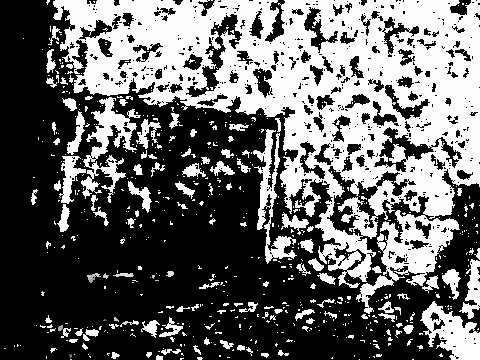
\includegraphics[width=45mm]{camera_tests/quad_camera_TX1}
  \caption{Depth image from RealSense that was mounted to quadcopter, with code running on TX1}
  \end{subfigure} %
  ~
  \begin{subfigure}[t]{0.3\textwidth}
  \centering
    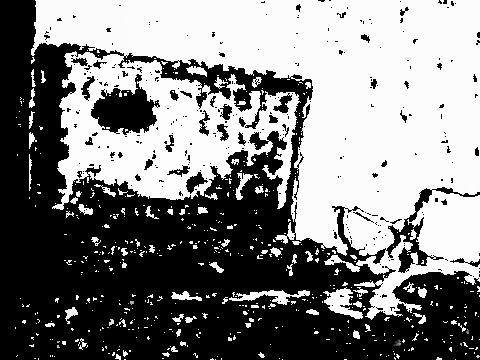
\includegraphics[width=45mm]{camera_tests/other_camera_TX1}
  \caption{Depth image from other RealSense, with code running on TX1}
  \end{subfigure}%
  ~
  \begin{subfigure}[t]{0.3\textwidth}
  \centering
    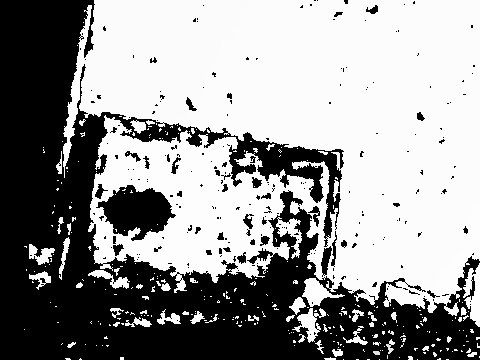
\includegraphics[width=45mm]{camera_tests/other_camera_ubuntu}
  \caption{Depth image from other RealSense, with code running on Ubuntu}
  \end{subfigure}
  \caption{Comparison of depth images for the two RealSense cameras and for running on different platforms.}
\end{figure}


\section{Stuff to do}
\begin{itemize}
\item Fix quadcopter
\item Adjust quadcopter trajectory so that it can see the top box
\item Investigate data
\begin{itemize}
\item \sout{Investigate boxes to determine which ones can be picked up as point clouds}
\item \sout{Investigate RealSense cameras, compare the two cameras and using them on TX1/TX2 or Windows/Ubuntu}
\end{itemize}
\item Investigate registration algorithm
\begin{itemize}
\item Generate 3D object in MATLAB that I can get points from from various camera poses (may also need to get RGB and depth images if we're going with that approach?)
\item Apply registration algorithm to generated point clouds (ground truth known) -- without noise first, then add noise. Get error in true and estimated translation and rotation.
\end{itemize}
\item Reading
\begin{itemize}
\item \sout{Incorporating RGB and depth images -- feature matching (papers you sent me)}
\item Write up summary of main points (parts of the algorithm, choices with advantages/disadvantages)
\item See if more recent papers have made advancements
\end{itemize}
\end{itemize}

\end{document}